\documentclass[aspectratio=169,10pt]{beamer}
\usetheme{Madrid}
\usecolortheme{default}
\setbeamertemplate{navigation symbols}{}
\setbeamertemplate{blocks}[rounded][shadow=false]
\usepackage{amsmath,amssymb,booktabs,mathtools,graphicx,tikz}
\usetikzlibrary{arrows.meta,positioning,calc}
\setbeamersize{text margin left=.6cm,text margin right=.6cm}
\definecolor{positive}{HTML}{0173B2}
\definecolor{negative}{HTML}{B22222}
\definecolor{emphasis}{HTML}{029E73}
\newcommand{\pos}[1]{\textcolor{positive}{#1}}
\newcommand{\warn}[1]{\textcolor{negative}{#1}}
\newcommand{\HL}[1]{\textcolor{emphasis}{#1}}
\newcommand{\R}{\mathbb R}
\newcommand{\Cset}{\mathcal C}
\newcommand{\src}[1]{\par\vspace{.5em}{\tiny\color{gray}#1\par}}
\setbeamertemplate{footline}{%
\begin{beamercolorbox}[wd=\paperwidth,ht=1.9ex,dp=.7ex,leftskip=.3cm,rightskip=.3cm]{section in head/foot}
\usebeamerfont{tiny}\hfill\insertsectionnavigationhorizontal{.9\paperwidth}{}{}\hfill
\end{beamercolorbox}%
\begin{beamercolorbox}[wd=\paperwidth,ht=2ex,dp=.9ex,leftskip=.3cm,rightskip=.3cm]{author in head/foot}
{\tiny\insertframenumber/\inserttotalframenumber\hfill Cheng et al.: Safe Reinforcement Learning with CBFs\hfill AAAI 2019}
\end{beamercolorbox}}
\tikzset{>=Stealth,box/.style={draw=positive!65,fill=positive!6,rounded corners=2pt,align=center,minimum height=.85cm,text width=2.5cm,font=\small},flow/.style={->,line width=.8pt,positive},data/.style={->,dashed,line width=.65pt,emphasis},lab/.style={font=\scriptsize,align=center}}
\title[Safe Reinforcement Learning with CBFs]{End-to-End Safe Reinforcement Learning through Barrier Functions for Safety-Critical Continuous Control Tasks}
\subtitle{Paper Review and Code Reproduction}
\author{Jinpeng Fan}
\institute{Southern University of Science and Technology}
\date{}
\begin{document}
% 1
\begin{frame}
\centering
{\color{positive}\large Paper Review and Code Reproduction\par}
\vspace{.8em}
\begin{beamercolorbox}[sep=.75em,center,rounded=true]{title}
\fontsize{18}{22}\selectfont
End-to-End Safe Reinforcement Learning through\\
Barrier Functions for Safety-Critical\\
Continuous Control Tasks
\end{beamercolorbox}
\vspace{1em}
{\small\color{gray}Original paper by\par}
\vspace{.3em}
{\normalsize Richard Cheng, G\'abor Orosz, Richard M. Murray, Joel W. Burdick\par}
\vspace{.35em}
{\small AAAI 2019\enspace\textbar\enspace arXiv:1903.08792v1\par}
\vspace{1.2em}
{\color{positive}\normalsize Presented by Jinpeng Fan\par}
\vspace{.3em}
{\small Southern University of Science and Technology\par}
\end{frame}
\section{Introduction}
% 2
\begin{frame}{Motivation}
\begin{enumerate}\setlength\itemsep{.9em}
\item Model-free reinforcement learning improves long-term return through exploration, but training actions can \warn{violate safety constraints before an effective policy is learned}.
\item Control barrier functions (CBFs) enforce safety constraints\textsuperscript{[1]}, but \warn{depend on a dynamics model and bounds on model error}.
\item Retaining past CBF corrections in later policy updates allows RL to improve the \warn{previously deployed safe controller}.
\end{enumerate}
\vspace{.6em}
\begin{block}{Objective}
Improve control performance through reinforcement learning while satisfying safety constraints during training under model uncertainty.
\end{block}
\vfill
{\fontsize{6.5}{8}\selectfont\color{gray}
[1] A. D. Ames, X. Xu, J. W. Grizzle, and P. Tabuada, ``Control Barrier Function Based Quadratic Programs for Safety Critical Systems,'' \emph{IEEE Transactions on Automatic Control}, vol. 62, no. 8, pp. 3861--3876, 2017.\par}
\end{frame}
\section{Problem Formulation}
% 4
\begin{frame}{Problem formulation}
Consider discrete-time, control-affine dynamics
\begin{equation}
s_{t+1}=f(s_t)+g(s_t)a_t+d(s_t),
\end{equation}
where $f,g$ define the nominal dynamics and $d(s_t)$ is the unknown state-dependent model residual.
\vspace{.5em}
\begin{columns}[T,onlytextwidth]
\begin{column}{.48\textwidth}
\begin{block}{Performance}
\begin{minipage}[t][2.15cm][t]{\linewidth}
\begin{minipage}[c][1.15cm][c]{\linewidth}
\centering
$\displaystyle\max_\pi J(\pi)=\mathbb E_{\tau\sim\pi}\!\left[\sum_{t=0}^{\infty}\gamma^t r(s_t,a_t)\right].$
\end{minipage}\par
Learn a policy that maximizes expected return from sampled trajectories.
\end{minipage}
\end{block}
\end{column}
\begin{column}{.48\textwidth}
\begin{block}{Safety}
\begin{minipage}[t][2.15cm][t]{\linewidth}
\begin{minipage}[c][1.15cm][c]{\linewidth}
\centering
$\displaystyle\Cset=\{s\in\R^n:h(s)\ge0\}.$
\end{minipage}\par
Keep the state in $\Cset$ throughout training, starting from $s_0\in\Cset$.
\end{minipage}
\end{block}
\end{column}
\end{columns}
\vspace{.5em}
The control input also satisfies $a_{\min}\le a_t\le a_{\max}$.
\end{frame}

% Policy-gradient background
\begin{frame}{Policy Gradient-Based RL: DDPG}
\small Deep Deterministic Policy Gradient
\begin{center}
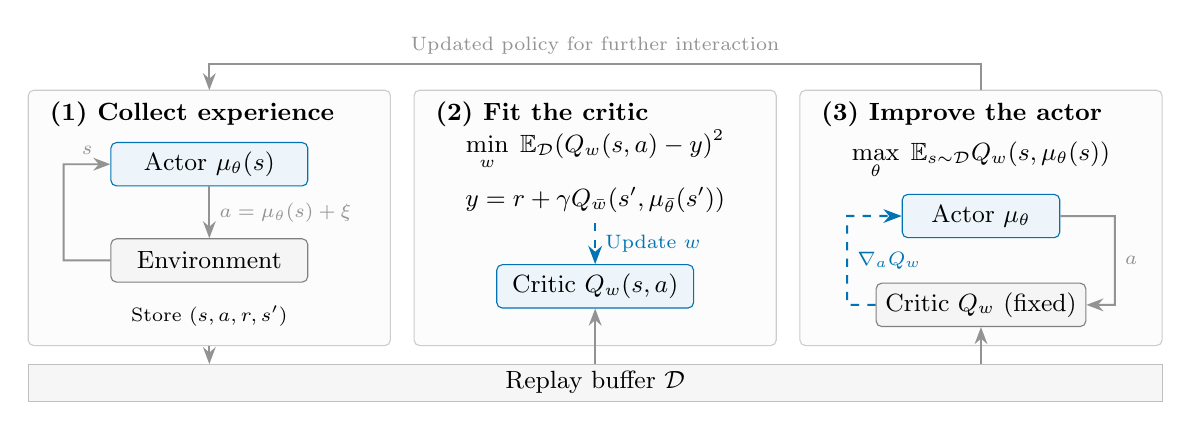
\begin{tikzpicture}[font=\small,yscale=.94,
 panel/.style={draw=gray!40,rounded corners=2pt,fill=gray!2},
 module/.style={draw=positive,fill=positive!7,rounded corners=2pt,align=center,minimum width=2.5cm,minimum height=.55cm},
 arr/.style={->,line width=.7pt,gray!85},
 grad/.style={->,dashed,line width=.8pt,positive}]
\foreach \x in {0,4.9,9.8}{\draw[panel] (\x,0) rectangle +(4.6,3.45);}
\node[anchor=west,font=\small\bfseries] at (.15,3.12) {(1) Collect experience};
\node[anchor=west,font=\small\bfseries] at (5.05,3.12) {(2) Fit the critic};
\node[anchor=west,font=\small\bfseries] at (9.95,3.12) {(3) Improve the actor};
\node[module] (policy) at (2.3,2.45) {Actor $\mu_\theta(s)$};
\node[module,draw=gray,fill=gray!8] (env) at (2.3,1.15) {Environment};
\draw[arr] (policy)--node[right,font=\scriptsize] {$a=\mu_\theta(s)+\xi$}(env);
\draw[arr] (env.west)--(.45,1.15)--(.45,2.45)--node[above,font=\scriptsize] {$s$}(policy.west);
\node[font=\scriptsize] at (2.3,.4) {Store $(s,a,r,s')$};
\node[align=center,font=\small] (loss) at (7.2,2.35)
 {$\displaystyle\min_w\;\mathbb E_{\mathcal D}(Q_w(s,a)-y)^2$\\[5pt]
 $y=r+\gamma Q_{\bar w}(s',\mu_{\bar\theta}(s'))$};
\node[module] (q) at (7.2,.8) {Critic $Q_w(s,a)$};
\draw[grad] (loss.south)--node[right,font=\scriptsize] {Update $w$}(q.north);
\node[align=center] at (12.1,2.5) {$\displaystyle\max_\theta\;\mathbb E_{s\sim\mathcal D}Q_w(s,\mu_\theta(s))$};
\node[module,minimum width=2cm] (act) at (12.1,1.75) {Actor $\mu_\theta$};
\node[module,minimum width=2cm,draw=gray,fill=gray!8] (fixedq) at (12.1,.55) {Critic $Q_w$ (fixed)};
\draw[arr] (act.east)--(13.8,1.75)--node[right,font=\scriptsize] {$a$}(13.8,.55)--(fixedq.east);
\draw[grad] (fixedq.west)--(10.4,.55)--node[right,font=\scriptsize] {$\nabla_a Q_w$}(10.4,1.75)--(act.west);
\draw[fill=gray!7,draw=gray!50] (0,-.75) rectangle (14.4,-.25);
\node (buffer) at (7.2,-.5) {Replay buffer $\mathcal D$};
\draw[arr] (2.3,0)--(2.3,-.25);
\draw[arr] (7.2,-.25)--(q.south);
\draw[arr] (12.1,-.25)--(fixedq.south);
\draw[arr] (12.1,3.45)--(12.1,3.8)--node[above,fill=white,font=\scriptsize] {Updated policy for further interaction}(2.3,3.8)--(2.3,3.45);
\end{tikzpicture}
\end{center}
\vspace{-.5em}
\begin{itemize}\setlength\itemsep{.2em}
\item \textbf{Off-policy:} reuse past transitions through minibatches from the replay buffer.
\item \textbf{Deterministic actor:} follow the critic's action gradient. Add noise for exploration.
\item \textbf{Target networks:} slowly updated $(\bar\theta,\bar w)$ stabilize the critic's targets.
\end{itemize}
\vfill
\src{T. P. Lillicrap et al., ``Continuous control with deep reinforcement learning,'' ICLR, 2016.}
\end{frame}

\begin{frame}{Policy Gradient-Based RL: TRPO}
\small Trust Region Policy Optimization
\begin{center}
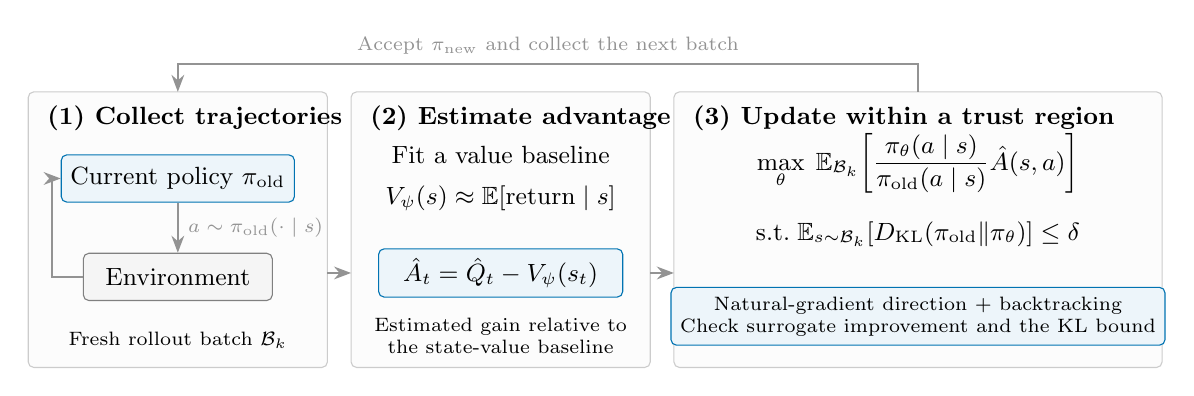
\begin{tikzpicture}[font=\small,
 panel/.style={draw=gray!40,rounded corners=2pt,fill=gray!2},
 module/.style={draw=positive,fill=positive!7,rounded corners=2pt,align=center,minimum width=2.4cm,minimum height=.6cm},
 arr/.style={->,line width=.7pt,gray!85}]
\draw[panel] (0,0) rectangle (3.8,3.5);
\draw[panel] (4.1,0) rectangle (7.9,3.5);
\draw[panel] (8.2,0) rectangle (14.4,3.5);
\node[anchor=west,font=\small\bfseries] at (.12,3.16) {(1) Collect trajectories};
\node[anchor=west,font=\small\bfseries] at (4.22,3.16) {(2) Estimate advantage};
\node[anchor=west,font=\small\bfseries] at (8.32,3.16) {(3) Update within a trust region};
\node[module] (policy) at (1.9,2.4) {Current policy $\pi_{\rm old}$};
\node[module,draw=gray,fill=gray!8] (env) at (1.9,1.15) {Environment};
\draw[arr] (policy)--node[right,font=\scriptsize] {$a\sim\pi_{\rm old}(\cdot\mid s)$}(env);
\draw[arr] (env.west)--(.3,1.15)--(.3,2.4)--(policy.west);
\node[font=\scriptsize] at (1.9,.35) {Fresh rollout batch $\mathcal B_k$};
\node[align=center] at (6,2.4) {Fit a value baseline\\[4pt] $V_\psi(s)\approx\mathbb E[\text{return}\mid s]$};
\node[module,minimum width=3.1cm] (adv) at (6,1.2) {$\hat A_t=\hat Q_t-V_\psi(s_t)$};
\node[align=center,font=\scriptsize] at (6,.4) {Estimated gain relative to\\the state-value baseline};
\draw[arr] (3.8,1.2)--(4.1,1.2);
\draw[arr] (7.9,1.2)--(8.2,1.2);
\node[align=center] at (11.3,2.25) {$\displaystyle\max_\theta\;\mathbb E_{\mathcal B_k}\!\left[\frac{\pi_\theta(a\mid s)}{\pi_{\rm old}(a\mid s)}\hat A(s,a)\right]$\\[9pt]
 $\displaystyle\text{s.t.}\;\mathbb E_{s\sim\mathcal B_k}\!\left[D_{\rm KL}(\pi_{\rm old}\|\pi_\theta)\right]\le\delta$};
\node[module,minimum width=5.4cm,font=\scriptsize] at (11.3,.65) {Natural-gradient direction + backtracking\\Check surrogate improvement and the KL bound};
\draw[arr] (11.3,3.5)--(11.3,3.85)--node[above,fill=white,font=\scriptsize] {Accept $\pi_{\rm new}$ and collect the next batch}(1.9,3.85)--(1.9,3.5);
\end{tikzpicture}
\end{center}
\vspace{-.2em}
\begin{itemize}\setlength\itemsep{.35em}
\item \textbf{On-policy:} collect a new batch with the current policy at each iteration.
\item \textbf{Stochastic policy:} increase the probability of actions with positive advantage.
\item \textbf{Trust region:} constrain the average KL divergence to limit policy changes.
\end{itemize}
\vfill
\src{J. Schulman et al., ``Trust Region Policy Optimization,'' ICML, 2015.}
\end{frame}

% Gaussian-process background
\begin{frame}{Gaussian Processes}
\small
\setlength{\abovedisplayskip}{5pt}
\setlength{\belowdisplayskip}{5pt}
Estimate the model residual $d(s)$ from recorded transitions:
\[
\hat d(s_t)=s_{t+1}-f(s_t)-g(s_t)a_t,\qquad a_t:\ \text{applied control input}.
\]
Fit a GP to each residual component, with a zero-mean prior, kernel $k$ and Gaussian noise variance $\sigma_{\rm noise}^2$.
\begin{block}{Posterior prediction}
\vspace{-.5em}
\begin{align*}
\mu_d(s)&=\mathbf k_s^\top(K+\sigma_{\rm noise}^2 I)^{-1}\mathbf y,\\[.2em]
\sigma_d^2(s)&=k(s,s)-\mathbf k_s^\top(K+\sigma_{\rm noise}^2 I)^{-1}\mathbf k_s.
\end{align*}
\vspace{-.2em}
{\small $K_{ij}=k(s_i,s_j)$,\quad $\mathbf k_s=[k(s_i,s)]_{i=1}^N$,\quad $\mathbf y=[\hat d(s_i)]_{i=1}^N$.\par\vspace{.3em}}
\end{block}
\vspace{-.1em}
\[
\text{GP confidence bounds:}\quad\boxed{\mu_d(s)-k_\delta\sigma_d(s)\le d(s)\le\mu_d(s)+k_\delta\sigma_d(s).}
\]
\vspace{-.5em}
\begin{itemize}\setlength\itemsep{.25em}
\item \textbf{Paper setting:} refit the GP between policy iterations using the latest $\approx 1{,}000$ transitions.
\item \textbf{Computational cost:} exact GP inference requires $\mathcal O(N^3)$ matrix factorization. Sparse or local GP approximations reduce this cost.
\end{itemize}
\vfill
\src{Cheng et al., AAAI 2019; C. E. Rasmussen and C. K. I. Williams, Gaussian Processes for Machine Learning, 2006.}
\end{frame}
\section{RL-CBF Method}
% CBF synthesis and safety
\begin{frame}{Control barrier functions}
\small
\setlength{\abovedisplayskip}{5pt}
\setlength{\belowdisplayskip}{5pt}
For $h(s)=p^\top s+q$ and $0\le\eta\le1$, the GP confidence bounds give the robust condition
\begin{equation}
\underbrace{p^\top[f(s_t)+g(s_t)a_t+\mu_d(s_t)]+q}_{\text{predicted next-step barrier value}}
-\underbrace{k_\delta|p|^\top\sigma_d(s_t)}_{\text{uncertainty margin}}
\ge(1-\eta)h(s_t).
\end{equation}
The CBF controller minimizes control effort while allowing a penalized safety slack:
\begin{equation}
\begin{aligned}
&(a_t^\star,\epsilon_t^\star)=\arg\min_{a_t,\,\epsilon\ge0}\;\tfrac12\|a_t\|_2^2+K_\epsilon\epsilon\\[.1em]
&\text{s.t.}\quad p^\top\!\left[f(s_t)+g(s_t)a_t+\mu_d(s_t)\right]+q-k_\delta|p|^\top\sigma_d(s_t)\ge(1-\eta)h(s_t)-\epsilon,\\[.1em]
&\phantom{\text{s.t.}\quad}a_{\rm low}\le a_t\le a_{\rm high}.
\end{aligned}
\end{equation}
The controller applies $a_t^\star$. The safety slack $\epsilon\ge0$ has penalty weight $K_\epsilon>0$.
\begin{block}{Safety guarantee}
\small
Assume the GP confidence bounds hold on the sets below and the required control inputs are feasible.
\begin{itemize}\setlength\itemsep{.1em}
\item If $\epsilon_t^\star=0$ throughout $\Cset$, then $s_0\in\Cset\Rightarrow s_t\in\Cset$ for all $t$.
\item If $\eta>0$ and $\epsilon_t^\star\le\bar\epsilon$ throughout $\Cset_{\bar\epsilon}$, then
$\Cset_{\bar\epsilon}=\{s:h(s)\ge-\bar\epsilon/\eta\}$ is forward invariant.
\end{itemize}
\end{block}
% Adapted from Eq. (9) and Lemma 1. Standard QP objective: squared control norm, nonnegative slack.
% Unlike the printed unsquared-norm objective, this is a quadratic program; the optimizer need not be identical.
% Squared correction convention: Ames et al., Control Barrier Functions: Theory and Applications, ECC 2019, Sec. II-C.
\end{frame}
% Adapted control optimization: Delta u_t is the decision variable; Delta u_t^star is its optimum.
% Quadratic correction cost and nonnegative slack; v_k substitutes the appropriate policy proposal.
\begin{frame}{CBF-Based Control with RL: Compensating}
\small
\setlength{\abovedisplayskip}{6pt}
\setlength{\belowdisplayskip}{6pt}
{\centering
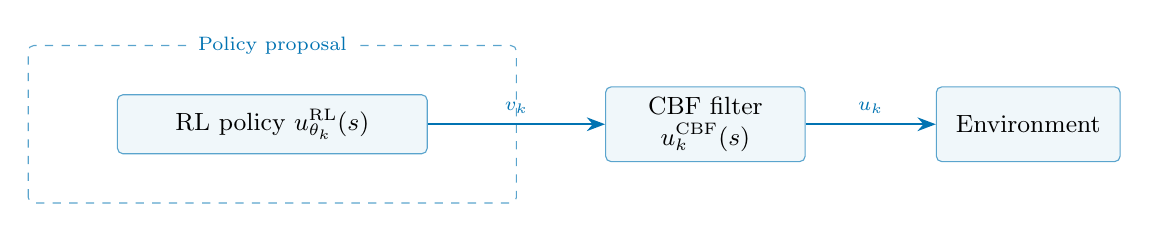
\begin{tikzpicture}[font=\small]
\draw[draw=positive!65,dashed,rounded corners=2pt] (0,-1.0) rectangle (6.2,1.0);
\node[font=\scriptsize,fill=white,text=positive] at (3.1,1.0) {Policy proposal};
\node[box,text width=3.7cm,minimum height=.75cm] (proposal) at (3.1,0) {RL policy $u^{\rm RL}_{\theta_k}(s)$};
\node[box,text width=2.3cm,minimum height=.95cm] (cbf) at (8.6,0) {CBF filter\\$u_k^{\rm CBF}(s)$};
\node[box,text width=2.1cm,minimum height=.95cm] (env) at (12.7,0) {Environment};
\draw[flow] (proposal.east)--node[above,lab] {$v_k$}(cbf.west);
\draw[flow] (cbf.east)--node[above,lab] {$u_k$}(env.west);
\end{tikzpicture}\par}
\vspace{.4em}
Proposal: $v_k=u^{\rm RL}_{\theta_k}$; applied input: $u_k=v_k+u_k^{\rm CBF}$.
\par The optimal correction $u_k^{\rm CBF}(s_t)=\Delta u_t^\star$ is obtained by solving the QP:
\begin{equation}
\begin{aligned}
&(\Delta u_t^\star,\epsilon_t^\star)=\arg\min_{\Delta u_t,\,\epsilon\ge0}\;\tfrac12\|\Delta u_t\|_2^2+K_\epsilon\epsilon\\[.1em]
&\text{s.t.}\quad p^\top\!\left[f(s_t)+g(s_t)\big(v_k(s_t)+\Delta u_t\big)+\mu_d(s_t)\right]+q-k_\delta|p|^\top\sigma_d(s_t)\ge(1-\eta)h(s_t)-\epsilon,\\[.1em]
&\phantom{\text{s.t.}\quad}a_{\rm low}\le v_k(s_t)+\Delta u_t\le a_{\rm high}.
\end{aligned}
\end{equation}
\begin{block}{Policy update}
\small
RL optimizes $u^{\rm RL}_{\theta_k}$, while the deployed controller is $u_k$.
The next proposal, $u^{\rm RL}_{\theta_{k+1}}$, does not explicitly retain past CBF corrections.
\end{block}
\end{frame}

% Adapted control optimization: Delta u_t is the decision variable; Delta u_t^star is its optimum.
% Quadratic correction cost and nonnegative slack; v_k substitutes the appropriate policy proposal.
\begin{frame}{CBF-Based Control with RL: Guiding}
\small
\setlength{\abovedisplayskip}{6pt}
\setlength{\belowdisplayskip}{6pt}
{\centering
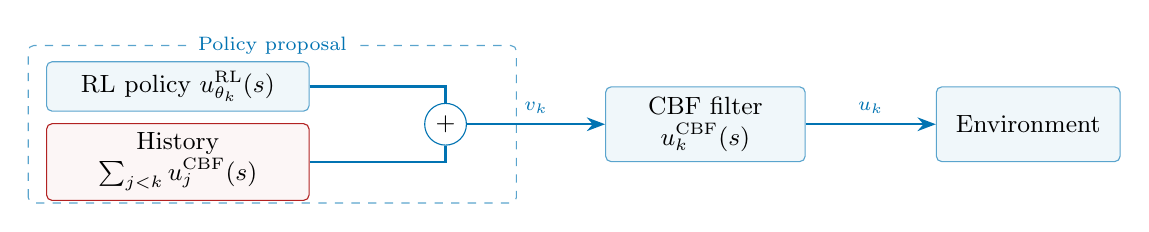
\begin{tikzpicture}[font=\small]
\draw[draw=positive!65,dashed,rounded corners=2pt] (0,-1.0) rectangle (6.2,1.0);
\node[font=\scriptsize,fill=white,text=positive] at (3.1,1.0) {Policy proposal};
\node[box,text width=3.1cm,minimum height=.5cm] (rl) at (1.9,.48) {RL policy $u^{\rm RL}_{\theta_k}(s)$};
\node[box,text width=3.1cm,minimum height=.5cm,draw=negative,fill=negative!4] (hist) at (1.9,-.48) {History $\sum_{j<k}u_j^{\rm CBF}(s)$};
\node[circle,draw=positive,inner sep=2pt] (proposal) at (5.3,0) {$+$};
\draw[line width=.8pt,positive] (rl.east)-|(proposal.north);
\draw[line width=.8pt,positive] (hist.east)-|(proposal.south);
\node[box,text width=2.3cm,minimum height=.95cm] (cbf) at (8.6,0) {CBF filter\\$u_k^{\rm CBF}(s)$};
\node[box,text width=2.1cm,minimum height=.95cm] (env) at (12.7,0) {Environment};
\draw[flow] (proposal.east)--node[above,lab] {$v_k$}(cbf.west);
\draw[flow] (cbf.east)--node[above,lab] {$u_k$}(env.west);
\end{tikzpicture}\par}
\vspace{.4em}
Proposal: $v_k=u^{\rm RL}_{\theta_k}+\sum_{j<k}u_j^{\rm CBF}$; applied input: $u_k=v_k+u_k^{\rm CBF}$.
\par The optimal correction $u_k^{\rm CBF}(s_t)=\Delta u_t^\star$ is obtained by solving the QP:
\begin{equation}
\begin{aligned}
&(\Delta u_t^\star,\epsilon_t^\star)=\arg\min_{\Delta u_t,\,\epsilon\ge0}\;\tfrac12\|\Delta u_t\|_2^2+K_\epsilon\epsilon\\[.1em]
&\text{s.t.}\quad p^\top\!\left[f(s_t)+g(s_t)\big(v_k(s_t)+\Delta u_t\big)+\mu_d(s_t)\right]+q-k_\delta|p|^\top\sigma_d(s_t)\ge(1-\eta)h(s_t)-\epsilon,\\[.1em]
&\phantom{\text{s.t.}\quad}a_{\rm low}\le v_k(s_t)+\Delta u_t\le a_{\rm high}.
\end{aligned}
\end{equation}
\begin{block}{Policy update}
\small
Retain the latest correction in the next proposal:
$v_{k+1}(s)=u^{\rm RL}_{\theta_{k+1}}(s)+\sum_{j=0}^{k}u_j^{\rm CBF}(s)$.
RL optimizes the proposal using the \warn{previously deployed controller} as a reference. The current CBF filter enforces safety.
\end{block}
\end{frame}
% 10
\begin{frame}{Efficient implementation}
Exact evaluation of all previous corrections requires storing historical policies and solving an increasing number of QPs.
\vspace{.6em}
\begin{block}{Compensation network}
A feedforward network approximates the accumulated CBF corrections:
\begin{equation}
b_{\phi_k}(s)\approx\sum_{j=0}^{k-1}u_j^{\rm CBF}(s),\qquad
u_k(s)=u^{\rm RL}_{\theta_k}(s)+b_{\phi_k}(s)+u_k^{\rm CBF}(s).
\end{equation}
\end{block}
\vspace{.5em}
\begin{enumerate}\setlength\itemsep{.6em}
\item Fit $b_{\phi_{k+1}}$ to the targets $b_{\phi_k}(s_t)+\Delta u_t^\star$ collected in iteration $k$.
\item Online control requires \pos{two network evaluations and one QP per step}, independent of the number of policy iterations.
\item The approximation changes the proposed input. The final CBF filter still enforces the safety constraints, but the approximation does not generally preserve the TRPO performance bound.
\end{enumerate}
% Source note: Computationally Efficient Algorithm and Algorithm 1.
\end{frame}
% Closed-loop implementation: explicit ports and unobstructed data paths.
\begin{frame}{Control architecture}
\centering
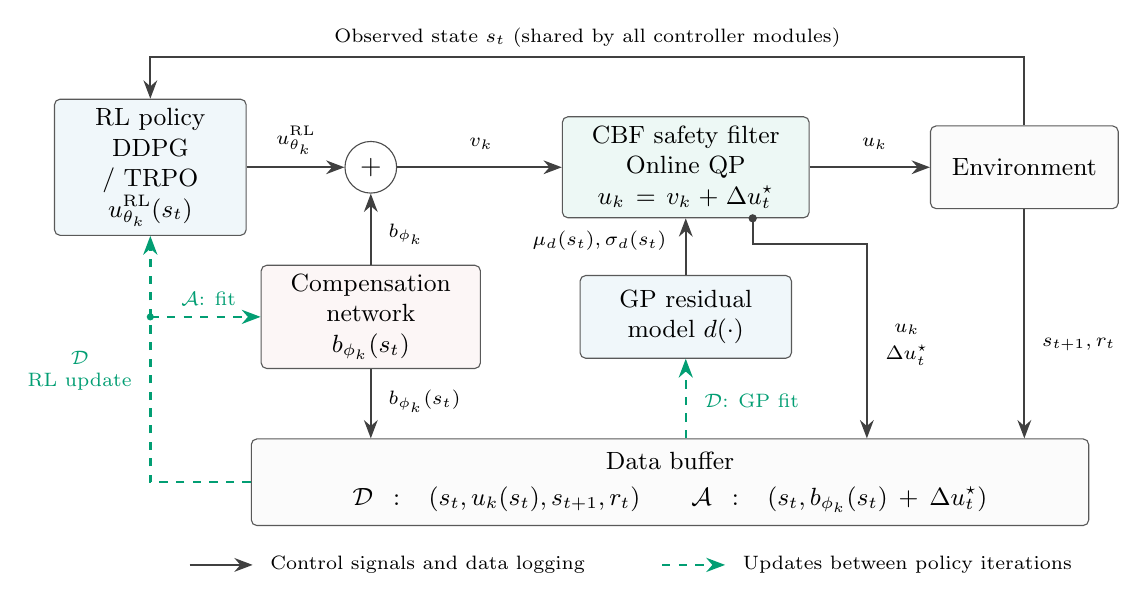
\begin{tikzpicture}[
 module/.style={draw=black!65,rounded corners=2pt,fill=gray!3,align=center,font=\small,minimum height=1.05cm},
 signal/.style={->,line width=.8pt,black!75},
 update/.style={->,dashed,line width=.85pt,emphasis},
 note/.style={font=\scriptsize,align=center,inner sep=0pt}]
% Online control. Labels are separate nodes, never opaque overlays on paths.
\node[module,text width=2.2cm,fill=positive!6] (rl) at (1.5,4.4)
 {RL policy\\DDPG / TRPO\\$u^{\rm RL}_{\theta_k}(s_t)$};
\node[circle,draw=black!70,inner sep=3pt] (sum) at (4.3,4.4) {$+$};
\node[module,text width=2.9cm,fill=emphasis!7] (cbf) at (8.3,4.4)
 {CBF safety filter\\Online QP\\$u_k=v_k+\Delta u_t^\star$};
\node[module,text width=2.15cm] (env) at (12.6,4.4) {Environment};
\node[module,text width=2.55cm,fill=negative!4] (comp) at (4.3,2.5)
 {Compensation network\\$b_{\phi_k}(s_t)$};
\node[module,text width=2.45cm,fill=positive!6] (gp) at (8.3,2.5)
 {GP residual\\model $d(\cdot)$};
\draw[signal] (rl.east)--(sum.west);
\node[note] at (3.35,4.74) {$u^{\rm RL}_{\theta_k}$};
\draw[signal] (comp.north)--(sum.south);
\node[note,anchor=west] at (4.52,3.55) {$b_{\phi_k}$};
\draw[signal] (sum.east)--(cbf.west);
\node[note] at (5.7,4.7) {$v_k$};
\draw[signal] (cbf.east)--(env.west);
\node[note] at (10.7,4.7) {$u_k$};
\draw[signal] (gp.north)--(cbf.south);
\node[note,anchor=east] at (8.06,3.47) {$\mu_d(s_t),\sigma_d(s_t)$};
% State feedback shared by all feedback modules.
\draw[signal] (env.north)--(12.6,5.8)--(1.5,5.8)--(rl.north);
\node[note] at (7.05,6.05) {Observed state $s_t$ (shared by all controller modules)};
% Buffer stores executed transitions and the next compensation target.
\node[module,text width=10.4cm,minimum height=1.1cm] (buffer) at (8.1,.4)
 {Data buffer\\[2pt]
 $\mathcal D:\ (s_t,u_k(s_t),s_{t+1},r_t)$\qquad
 $\mathcal A:\ (s_t,b_{\phi_k}(s_t)+\Delta u_t^\star)$};
\draw[signal] (env.south)--(env.south |- buffer.north);
\node[note,anchor=west] at (12.82,2.15) {$s_{t+1},r_t$};
% Dedicated logging port on the filter's lower edge: no ambiguous corner branch.
\coordinate (logport) at ($(cbf.south)+(.85,0)$);
\coordinate (logturn) at (10.6,3.43);
\draw[signal] (logport)--(logport |- logturn)--(logturn)--(logturn |- buffer.north);
\fill[black!75] (logport) circle (1.5pt);
\node[note,anchor=west] at (10.83,2.15) {$u_k$\\[2pt]$\Delta u_t^\star$};
\draw[signal] (comp.south)--(comp.south |- buffer.north);
\node[note,anchor=west] at (4.52,1.43) {$b_{\phi_k}(s_t)$};
% Iteration updates use separate corridors and exact module anchors.
\draw[update] (buffer.west)--(1.5,.4)--(rl.south);
\node[note,anchor=east,text=emphasis] at (1.27,1.82) {$\mathcal D$\\RL update};
\draw[update] (1.5,2.5)--(comp.west);
\node[note,text=emphasis] at (2.24,2.73) {$\mathcal A$: fit};
\fill[emphasis] (1.5,2.5) circle (1.3pt);
\draw[update] (gp.south |- buffer.north)--(gp.south);
\node[note,anchor=west,text=emphasis] at (8.53,1.43) {$\mathcal D$: GP fit};
\draw[signal] (2,-.65)--(2.8,-.65);
\node[anchor=west,font=\scriptsize] at (2.9,-.65) {Control signals and data logging};
\draw[update] (8,-.65)--(8.8,-.65);
\node[anchor=west,font=\scriptsize] at (8.9,-.65) {Updates between policy iterations};
\end{tikzpicture}
\end{frame}
% 11
\section{Simulation Results}
% 12: overview only. Implementation details remain in the reproduction report.
\begin{frame}{Reproduction overview}
\small
We corrected implementation errors and revised the modeling and experimental settings in the original code. The following results focus on the revised implementation, with original-code reruns for comparison. The reproduction report details the changes.
\vspace{.35em}
\begin{center}
\renewcommand{\arraystretch}{1.23}
\begin{tabular}{@{}lll@{}}
\toprule
Task & Training per seed & Safety constraint\\\midrule
Inverted pendulum & 600 episodes, 200 steps each & $|\theta|\le1$ rad\\
Car following (5 cars) & $3\times10^5$ steps & Car 4: front/rear gaps $\ge2$ m\\
\bottomrule
\end{tabular}
\end{center}
Four algorithms, seeds 1--3. Within each seed, algorithms share the environment and initial-state sequences. Car runs also share the acceleration-noise sequences.
\par\vspace{.45em}
\noindent\pos{\textbf{Reruns of the original code}}\par
\begin{itemize}\setlength\itemsep{.4em}
\item \textbf{Pendulum:} in the first 600 episodes, TRPO-CBF recorded 1, 9 and 332 violating episodes across seeds 1--3. DDPG-CBF recorded 37--127 and continued to rely on CBF corrections.
\item \textbf{Car following:} both CBF variants avoided collisions, but the gap fell below 2 m in 12 episodes. DDPG-CBF did not converge.
\end{itemize}
% Sources: reproduction report, Sections 1--3 and Supplement C.
\end{frame}

% 13. Sources: report Fig. 1 / Table 3 and figures/pendulum_metrics.json.
\begin{frame}{Inverted pendulum: training results}
\begin{columns}[c,onlytextwidth]
\begin{column}{.58\textwidth}
\centering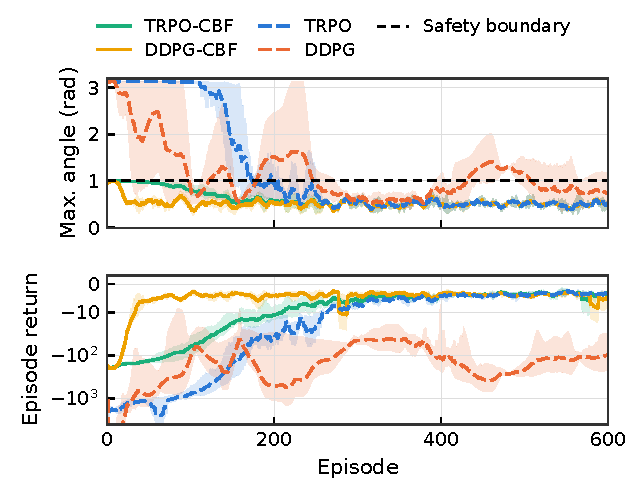
\includegraphics[width=\linewidth]{images/repro_pendulum_training.pdf}
\end{column}
\begin{column}{.40\textwidth}
\small
\pos{\textbf{Safety}}
\par TRPO-CBF: \textbf{0/1800} violating episodes.
\par DDPG-CBF: \textbf{1/1800}, in seed 3, episode 7, with positive slack.
\par\vspace{.55em}
\noindent\pos{\textbf{Learning speed}}
\par{\scriptsize Episodes to the first 20-episode mean return above $-10$.\par}
\vspace{.2em}
\begin{tabular}{@{}lr@{}}
\toprule
DDPG-CBF & 36--45\\
TRPO-CBF & 157--244\\
TRPO & 264--268\\
DDPG & Not reached\\
\bottomrule
\end{tabular}
\vspace{.55em}
\par\pos{\textbf{Comparable final returns}}
\par TRPO: $-3.33$\qquad TRPO-CBF: $-3.52$.
\par{\scriptsize Mean over the last 100 episodes.\par}
\end{column}
\end{columns}
\src{Revised code, seeds 1--3. Curves use 10-episode smoothing. Lines show seed means, shading the min--max range. Return axis: symmetric log scale.}
\end{frame}

% 14. Source: report Fig. 2; pendulum/results/checkpoint_rerun_seed1/.
% Initial: untrained policy, zero compensation and GP prior.
% Final: trained policy/compensation and final GP posterior. Each GP is frozen during evaluation.
\begin{frame}{Inverted pendulum: closed-loop evaluation}
\small
We compare the untrained and final policies from the same ten initial states (seed 1), using deterministic actions for 10 s per rollout. Each stage uses its corresponding compensation network and GP, with no GP updates during evaluation.
\par\vspace{.3em}
\centering
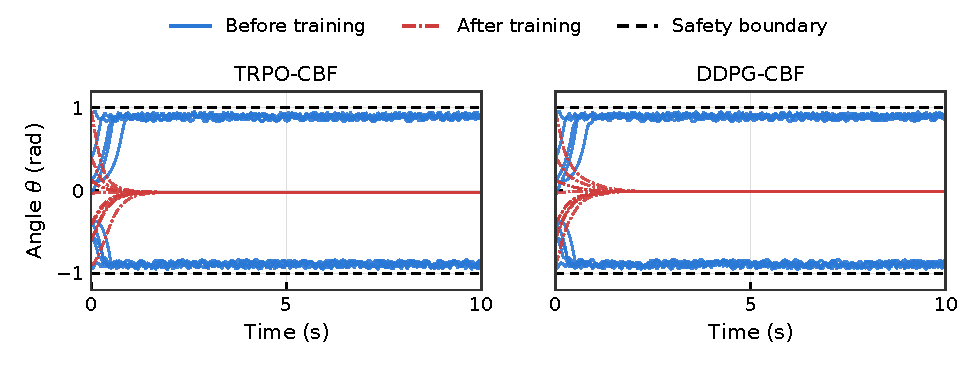
\includegraphics[width=10.0cm]{images/repro_pendulum_policies.pdf}\par
\vspace{.15em}
\begin{columns}[T,onlytextwidth]
\begin{column}{.47\textwidth}
\small\pos{\textbf{Before training}}
\par CBF corrections keep the pendulum near $|\theta|\approx0.9$ rad.
\end{column}
\begin{column}{.49\textwidth}
\small\pos{\textbf{After training}}
\par Upright within 1--2 s, with $u^{\rm CBF}=0$ throughout evaluation.
\end{column}
\end{columns}
\vspace{.45em}
{\footnotesize Training correction RMS: 3.3 to 0.02 N\,$\cdot$\,m (TRPO-CBF), 3.7 to 0.01 N\,$\cdot$\,m (DDPG-CBF).\par}
\end{frame}

% 15. Sources: report Fig. 3 / Table 4 and figures/car_metrics.json.
\begin{frame}{Car following: training results}
\begin{columns}[c,onlytextwidth]
\begin{column}{.58\textwidth}
\centering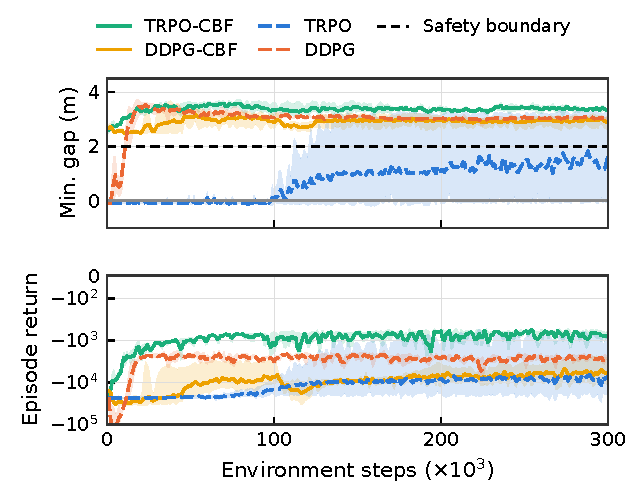
\includegraphics[width=\linewidth]{images/repro_car_training.pdf}
\end{column}
\begin{column}{.40\textwidth}
\small
\pos{\textbf{Safety}}
\par Both CBF variants: no collisions or 2 m gap violations.
\par Minimum gap: \textbf{2.33 m}.
\par\vspace{.55em}
\noindent\pos{\textbf{Learning speed}}
\par First 50-episode mean return above $-5000$:
\par TRPO-CBF: \textbf{11,000--14,000} steps.
\par DDPG: 20,000--23,000 steps.
\par Final TRPO-CBF return: $-740$.
\par\vspace{.55em}
\noindent\pos{\textbf{DDPG-CBF}}
\par Lower final return than DDPG: $-5856$ vs. $-2586$.
\par Compensation RMS: 92--98 m/s$^2$, near the $\pm100$ limit.
\end{column}
\end{columns}
\src{Revised code, seeds 1--3. Curves: 10-episode smoothing, seed mean and min--max range. Final return: last 100 episodes. Return axis: symmetric log scale.}
\end{frame}

% 16. Sources: report Fig. 4 / Supplement C.2 and figures/car_final_sim.json.
% All three response variables retained, with a horizontal plot arrangement for projection.
\begin{frame}{Car following: closed-loop evaluation}
\small
We compare the final policies as the front car slows down. Each 10 s simulation uses deterministic actions, a common initial state and noise sequence, and fixed GP models. The plots show seed 1.
\par\vspace{.3em}
\centering
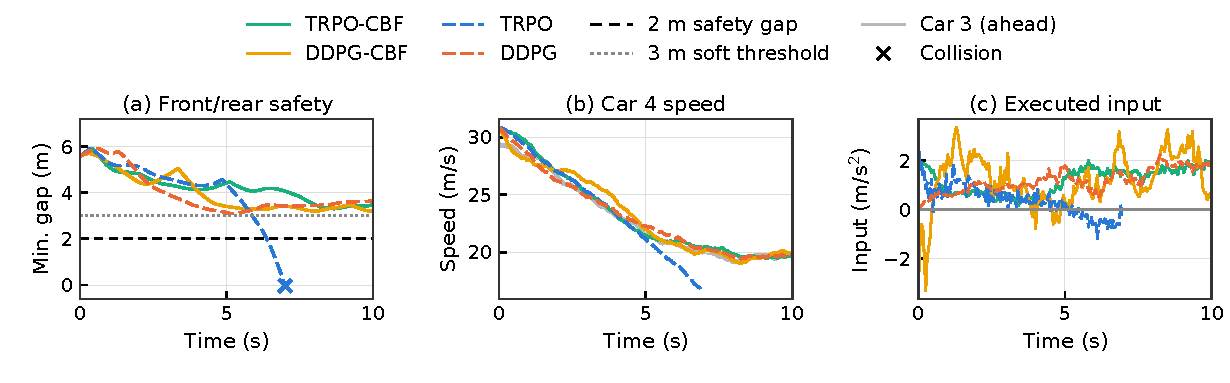
\includegraphics[width=\textwidth]{images/repro_car_policies.pdf}\par
\vspace{.1em}
\begin{columns}[T,onlytextwidth]
\begin{column}{.48\textwidth}
\small\pos{\textbf{Seed 1}}
\par Minimum gaps are 3.1--3.3 m for both CBF variants and DDPG. TRPO is rear-ended at 7.0 s.
\end{column}
\begin{column}{.48\textwidth}
\small\pos{\textbf{Across seeds}}
\par TRPO-CBF needs no CBF correction in any seed. DDPG-CBF needs it in 62\% of steps (seed 2) and 55\% (seed 3).
\end{column}
\end{columns}
% The full protocol (recalibration and five GP warm-up episodes) is in Supplement C.2.
\end{frame}

\section{Conclusions}
% 17. These are reproduction findings, not a restatement of the paper's claims.
\begin{frame}{Conclusions}
\begin{enumerate}\setlength\itemsep{.8em}
\item \textbf{Training safety.} Both car-following CBF variants remained collision-free. Pendulum TRPO-CBF had no violations, while DDPG-CBF had one early violation.
\item \textbf{Learning speed and final return.} Both pendulum CBF variants and car-following TRPO-CBF reached return thresholds earlier. Final returns were not consistently higher than the baselines.
\item \textbf{CBF corrections and compensation.} CBF corrections became negligible for both pendulum variants and car-following TRPO-CBF. Car-following DDPG-CBF showed compensation saturation and underperformed DDPG.
\end{enumerate}
\vspace{.6em}
\begin{block}{Comparison scope}
\small
Car dynamics, reward and episode length changed, so returns cannot be compared directly with the paper. The experiments do not isolate individual changes through ablations.
\end{block}
\src{Sources: reproduction report, Sections 3--4 and Supplement C. These findings refer to the revised implementation.}
\end{frame}


% 18. Two approved theory topics are retained verbatim; only the application changes.
% No visible references, per the user request.
% Application background: Yang et al., CBF-RL, ICRA 2026,
% DOI: 10.1109/ICRA57385.2026.11695808; arXiv:2510.14959.
% The paper demonstrates training-time filtering/reward shaping and humanoid
% obstacle avoidance/stair climbing without a runtime filter. Its analysis concerns
% filtered reduced-order dynamics; the proposed research investigates deployment
% safety under changed conditions, policy verification and lightweight online protection.
% These are proposed directions, not completed results or claims of novelty.
\begingroup
\setbeamertemplate{footline}{%
\begin{beamercolorbox}[wd=\paperwidth,ht=1.9ex,dp=.7ex,leftskip=.3cm,rightskip=.3cm]{section in head/foot}
\usebeamerfont{tiny}\hfill\insertsectionnavigationhorizontal{.9\paperwidth}{}{}\hfill
\end{beamercolorbox}%
\begin{beamercolorbox}[wd=\paperwidth,ht=2ex,dp=.9ex,leftskip=.3cm,rightskip=.3cm]{author in head/foot}
{\tiny\insertframenumber/\inserttotalframenumber\hfill Proposed PhD Research: Safe RL with CBFs\hfill Jinpeng Fan}
\end{beamercolorbox}}

\begin{frame}{Research plan: safety-guaranteed reinforcement learning}
\pos{\textbf{Goal:}} develop RL methods with safety and convergence guarantees for robotic systems.
\par\vspace{.75em}
\begin{enumerate}\setlength\itemsep{1.2em}
\item \textbf{Theory: policy optimization and convergence}\par\vspace{.2em}
Study how CBF safety filtering affects policy updates and convergence. Develop learning rules that improve control performance while satisfying safety constraints.
\item \textbf{Theory: safety guarantees under model uncertainty}\par\vspace{.2em}
Study how limited data and model errors affect CBF safety guarantees. Establish conditions for maintaining feasibility when several safety constraints must be satisfied at the same time.
\item \textbf{Application: safe humanoid locomotion}\par\vspace{.2em}
Evaluate policies trained with CBFs on humanoids under changing terrain, payloads and sensing errors. Develop policy verification methods and lightweight online safeguards to improve deployment safety while meeting real-time constraints.
\end{enumerate}
\end{frame}
\endgroup
\end{document}
